\ifdefined\included
\else
\documentclass[english,a4paper,11pt,twoside]{StyleThese}
\usepackage{amsmath,amssymb}             % AMS Math
\usepackage[T1]{fontenc}
\usepackage[utf8x]{inputenc}
\usepackage{babel}
\usepackage{datetime}

\usepackage{lmodern}
\usepackage{tabularx}
%\usepackage{tabular}
\usepackage{multirow}

\usepackage{subfigure}
\usepackage{fancyvrb}


\usepackage{hhline}
\usepackage[left=1.5in,right=1.3in,top=1.1in,bottom=1.1in,includefoot,includehead,headheight=13.6pt]{geometry}
\renewcommand{\baselinestretch}{1.05}

% Table of contents for each chapter

\usepackage[nottoc, notlof, notlot]{tocbibind}
\usepackage{minitoc}
\setcounter{minitocdepth}{2}
\mtcindent=15pt
% Use \minitoc where to put a table of contents

\usepackage{aecompl}


% Glossary / list of abbreviations

\usepackage[intoc]{nomencl}
\iftoggle{ThesisInEnglish}{%
\renewcommand{\nomname}{Glossary}
}{ %
\renewcommand{\nomname}{Liste des Abréviations}
}

\makenomenclature

% My pdf code

\usepackage{ifpdf}

\ifpdf
  \usepackage[pdftex]{graphicx}
  \DeclareGraphicsExtensions{.jpg}
  \usepackage[a4paper,pagebackref,hyperindex=true]{hyperref}
  \usepackage{tikz}
  \usetikzlibrary{arrows,shapes,calc}
\else
  \usepackage{graphicx}
  \DeclareGraphicsExtensions{.ps,.eps}
  \usepackage[a4paper,dvipdfm,pagebackref,hyperindex=true]{hyperref}
\fi

\graphicspath{{.}{images/}}

%% nicer backref links. NOTE: The flag ThesisInEnglish is used to define the
% language in the back references. Read more about it in These.tex

\iftoggle{ThesisInEnglish}{%
\renewcommand*{\backref}[1]{}
\renewcommand*{\backrefalt}[4]{%
\ifcase #1 %
(Not cited.)%
\or
(Cited in page~#2.)%
\else
(Cited in pages~#2.)%
\fi}
\renewcommand*{\backrefsep}{, }
\renewcommand*{\backreftwosep}{ and~}
\renewcommand*{\backreflastsep}{ and~}
}{%
\renewcommand*{\backref}[1]{}
\renewcommand*{\backrefalt}[4]{%
\ifcase #1 %
(Non cité.)%
\or
(Cité en page~#2.)%
\else
(Cité en pages~#2.)%
\fi}
\renewcommand*{\backrefsep}{, }
\renewcommand*{\backreftwosep}{ et~}
\renewcommand*{\backreflastsep}{ et~}
}

% Links in pdf
\usepackage{color}
\definecolor{linkcol}{rgb}{0,0,0.4} 
\definecolor{citecol}{rgb}{0.5,0,0} 
\definecolor{linkcol}{rgb}{0,0,0} 
\definecolor{citecol}{rgb}{0,0,0}
% Change this to change the informations included in the pdf file

\hypersetup
{
bookmarksopen=true,
pdftitle="Joint Action for Human-Robot Interaction",
pdfauthor="Sandra DEVIN", %auteur du document
pdfsubject="Thesis", %sujet du document
%pdftoolbar=false, %barre d'outils non visible
pdfmenubar=true, %barre de menu visible
pdfhighlight=/O, %effet d'un clic sur un lien hypertexte
colorlinks=true, %couleurs sur les liens hypertextes
pdfpagemode=None, %aucun mode de page
pdfpagelayout=SinglePage, %ouverture en simple page
pdffitwindow=true, %pages ouvertes entierement dans toute la fenetre
linkcolor=linkcol, %couleur des liens hypertextes internes
citecolor=citecol, %couleur des liens pour les citations
urlcolor=linkcol %couleur des liens pour les url
}

% definitions.
% -------------------

\setcounter{secnumdepth}{3}
\setcounter{tocdepth}{2}

% Some useful commands and shortcut for maths:  partial derivative and stuff

\newcommand{\pd}[2]{\frac{\partial #1}{\partial #2}}
\def\abs{\operatorname{abs}}
\def\argmax{\operatornamewithlimits{arg\,max}}
\def\argmin{\operatornamewithlimits{arg\,min}}
\def\diag{\operatorname{Diag}}
\newcommand{\eqRef}[1]{(\ref{#1})}

\usepackage{rotating}                    % Sideways of figures & tables
%\usepackage{bibunits}
%\usepackage[sectionbib]{chapterbib}          % Cross-reference package (Natural BiB)
%\usepackage{natbib}                  % Put References at the end of each chapter
                                         % Do not put 'sectionbib' option here.
                                         % Sectionbib option in 'natbib' will do.
\usepackage{fancyhdr}                    % Fancy Header and Footer

% \usepackage{txfonts}                     % Public Times New Roman text & math font
  
%%% Fancy Header %%%%%%%%%%%%%%%%%%%%%%%%%%%%%%%%%%%%%%%%%%%%%%%%%%%%%%%%%%%%%%%%%%
% Fancy Header Style Options

\pagestyle{fancy}                       % Sets fancy header and footer
\fancyfoot{}                            % Delete current footer settings

%\renewcommand{\chaptermark}[1]{         % Lower Case Chapter marker style
%  \markboth{\chaptername\ \thechapter.\ #1}}{}} %

%\renewcommand{\sectionmark}[1]{         % Lower case Section marker style
%  \markright{\thesection.\ #1}}         %

\fancyhead[LE,RO]{\bfseries\thepage}    % Page number (boldface) in left on even
% pages and right on odd pages
\fancyhead[RE]{\bfseries\nouppercase{\leftmark}}      % Chapter in the right on even pages
\fancyhead[LO]{\bfseries\nouppercase{\rightmark}}     % Section in the left on odd pages

\let\headruleORIG\headrule
\renewcommand{\headrule}{\color{black} \headruleORIG}
\renewcommand{\headrulewidth}{1.0pt}
\usepackage{colortbl}
\arrayrulecolor{black}

\fancypagestyle{plain}{
  \fancyhead{}
  \fancyfoot{}
  \renewcommand{\headrulewidth}{0pt}
}

%\usepackage{MyAlgorithm}
%\usepackage[noend]{MyAlgorithmic}
\usepackage[ED=MITT - STICIA, Ets=INP]{tlsflyleaf}
%%% Clear Header %%%%%%%%%%%%%%%%%%%%%%%%%%%%%%%%%%%%%%%%%%%%%%%%%%%%%%%%%%%%%%%%%%
% Clear Header Style on the Last Empty Odd pages
\makeatletter

\def\cleardoublepage{\clearpage\if@twoside \ifodd\c@page\else%
  \hbox{}%
  \thispagestyle{empty}%              % Empty header styles
  \newpage%
  \if@twocolumn\hbox{}\newpage\fi\fi\fi}

\makeatother
 
%%%%%%%%%%%%%%%%%%%%%%%%%%%%%%%%%%%%%%%%%%%%%%%%%%%%%%%%%%%%%%%%%%%%%%%%%%%%%%% 
% Prints your review date and 'Draft Version' (From Josullvn, CS, CMU)
\newcommand{\reviewtimetoday}[2]{\special{!userdict begin
    /bop-hook{gsave 20 710 translate 45 rotate 0.8 setgray
      /Times-Roman findfont 12 scalefont setfont 0 0   moveto (#1) show
      0 -12 moveto (#2) show grestore}def end}}
% You can turn on or off this option.
% \reviewtimetoday{\today}{Draft Version}
%%%%%%%%%%%%%%%%%%%%%%%%%%%%%%%%%%%%%%%%%%%%%%%%%%%%%%%%%%%%%%%%%%%%%%%%%%%%%%% 

\newenvironment{maxime}[1]
{
\vspace*{0cm}
\hfill
\begin{minipage}{0.5\textwidth}%
%\rule[0.5ex]{\textwidth}{0.1mm}\\%
\hrulefill $\:$ {\bf #1}\\
%\vspace*{-0.25cm}
\it 
}%
{%

\hrulefill
\vspace*{0.5cm}%
\end{minipage}
}

\let\minitocORIG\minitoc
\renewcommand{\minitoc}{\minitocORIG \vspace{1.5em}}

\usepackage{multirow}
%\usepackage{slashbox}

\newenvironment{bulletList}%
{ \begin{list}%
	{$\bullet$}%
	{\setlength{\labelwidth}{25pt}%
	 \setlength{\leftmargin}{30pt}%
	 \setlength{\itemsep}{\parsep}}}%
{ \end{list} }

\newtheorem{definition}{Définition}
\renewcommand{\epsilon}{\varepsilon}

% centered page environment

\newenvironment{vcenterpage}
{\newpage\vspace*{\fill}\thispagestyle{empty}\renewcommand{\headrulewidth}{0pt}}
{\vspace*{\fill}}

\usepackage{tablefootnote}

\sloppy
\begin{document}
\setcounter{chapter}{1} %% Numéro du chapitre précédent ;)
\dominitoc
\faketableofcontents
\fi

\chapter{Supervision for Human-Robot Interaction}
\minitoc

\label{ch:Sup}

\section{Role of the supervisor in the global architecture}

One of the goal of the research group in which one I was integrated at LAAS-CNRS is to build a fully autonomous robot which interacts and performs Joint Actions with humans. To do so, an architecture for human-robot interaction has been developed and is constantly improved. This architecture is composed of several modules and a simplified scheme of it can be found in Fig.~\ref{fig:GlobalArchi}.

\begin{figure}[!h]
	\centering
    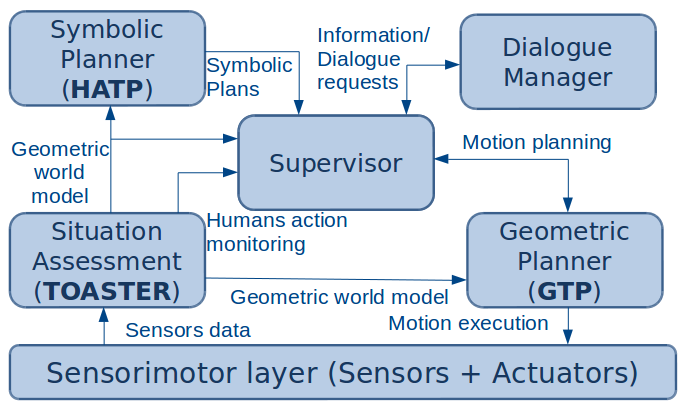
\includegraphics[width=0.7\textwidth]{figs/Chapter2/archiGlobal.png}
    \caption{The global architecture for human-robot interaction implemented at LAAS-CNRS.}
    \label{fig:GlobalArchi}
\end{figure}

\paragraph{Sensorimotor layer:}
The lower level of the architecture is composed of modules which allow to communicate and control sensors and actuators. Among others, this layer is composed of modules interpreting sensors data to detect humans and objects and a module allowing to execute given trajectories by calling the adequate actuators.

\paragraph{Situation Assessment:}
The situation assessment is done by a soft called TOASTER \cite{milliezThesis}. One of the functionalities of TOASTER is to build and maintain a consistent world state based on data coming from the sensorimotor layer. Geometrics computation are done on this world state to compute symbolic predicates concerning the environment (e.g. \textit{<object, isOn, support>}, \textit{<object, isIn, box>}) and agents abilities and behavior (e.g. \textit{object, isVisibleBy, human}, \textit{<object, isReachableBy, robot>}, \textit{human, isLookingToward, object}). TOASTER is also in charge of perspective taking: the previous predicates are contently estimated and maintained from the point of view of all humans.

\paragraph{Geometric Planner:}
In order to perform actions and movements adapted to the human proximity, our architecture is equipped with a geometric task and motion planner called GTP \cite{waldhart2016novel}. GTP allows to compute trajectories as well as objects placements and grasps in order to refine actions such as Pick or Place while taking into account the human safety and comfort.

\paragraph{Symbolic Planner:}
For the robot to be able to synthesize Shared Plans, our architecture is equipped with HATP, a human-aware HTN (Hierarchical Task Network) task planner which allows the robot to compute and refine a plan both for itself and its humans partners, taking into account a number of social rules \cite{Lallement2014hatp}.

HATP has been specially designed to integrate a number of features that are meant to promote the synthesis of plans that are acceptable by humans and easily if not trivially understandable by them. It allows to specify the humans and robot capabilities in terms of actions they can execute. Several aspects such as human preferences and comfort, estimation of human effort to achieve a task in a given context and "social rules" are used in a cost-based approach to build "sufficiently good" human-robot Shared Plans.

\paragraph{Dialogue Manager:}
In order for the robot to communicate with humans, a basic dialogue manager has been integrated to the architecture. This module allows to give humans information, ask basic questions and understand basic answers.

\paragraph{Supervisor:}
The last module of the architecture is the supervisor. It is the one in charge of controlling collaborative activities. It chooses the robot goals and monitors the Shared Plan execution. To do so, it estimates humans mental states concerning the Shared Plan and takes them into account to decide when to perform actions or to communicate (verbally and/or non-verbally). It also interprets the information coming from the Situation Assessment module in order to recognize human actions like Pick or Place with regard to the Shared Plan. This module is an extension of \cite{clodic2009shary} and \cite{fiore2016planning} and is the major technical contribution of the thesis. Its internal architecture will be detailed in the next section.

\section{The supervisor architecture}

The supervisor is composed of several modules and is fully implemented in ROS\footnote{http://www.ros.org/}. The complete scheme of its architecture can be found in Fig.~\ref{fig:archiSup}, however, as the figure is quite complex, each composing part of the supervisor will be described individually in the next subsections. 

\begin{figure}[!h]
	\centering
    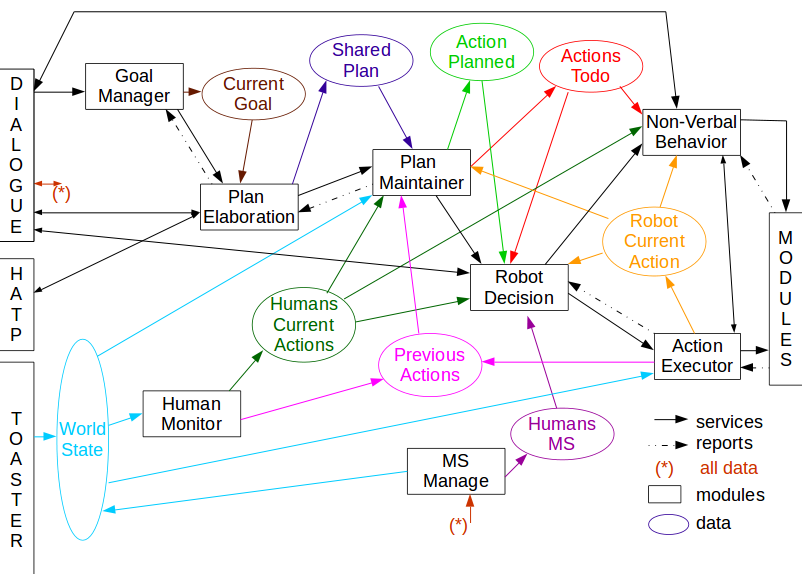
\includegraphics[width=\textwidth]{figs/Chapter2/ArchiSup.png}
    \caption{Architecture of the supervisor.}
    \label{fig:archiSup}
\end{figure}

\subsection{Goal Manager}

\begin{figure}[!h]
	\centering
    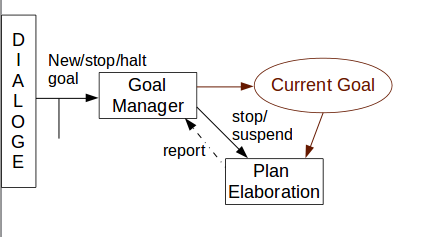
\includegraphics[width=0.5\textwidth]{figs/Chapter2/GoalManager.png}
    \caption{Interaction of the Goal Manager with the rest of the supervisor.}
    \label{fig:goalManager}
\end{figure}

\subsection{Plan elaboration}

\begin{figure}[!h]
	\centering
    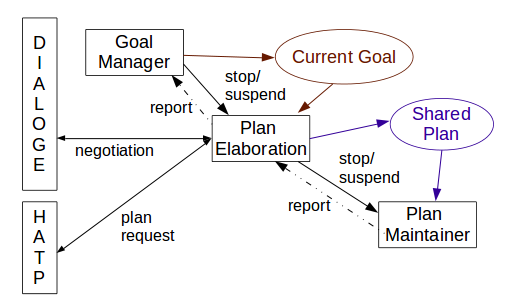
\includegraphics[width=0.6\textwidth]{figs/Chapter2/PlanElaboration.png}
    \caption{Interaction of the Plan Elaboration module with the rest of the supervisor.}
    \label{fig:planElaboration}
\end{figure}

\subsection{Plan Maintainer}

\begin{figure}[!h]
	\centering
    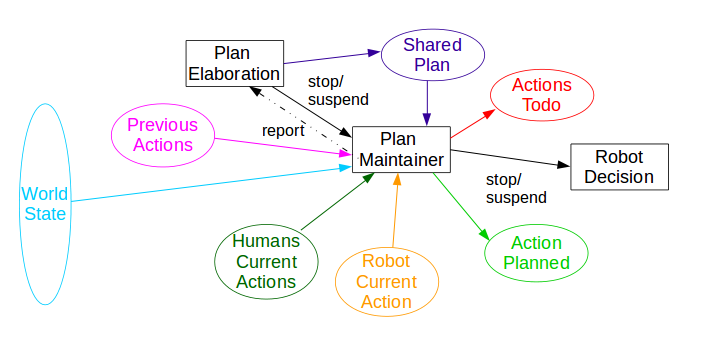
\includegraphics[width=0.8\textwidth]{figs/Chapter2/PlanMaintainer.png}
    \caption{Interaction of the Plan Maintainer with the rest of the supervisor.}
    \label{fig:planMaintainer}
\end{figure}

\subsection{Human Monitor}

\begin{figure}[!h]
	\centering
    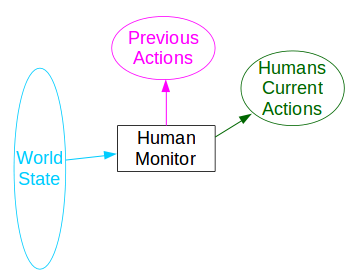
\includegraphics[width=0.4\textwidth]{figs/Chapter2/HumanMonitor.png}
    \caption{Interaction of the Human Monitor module with the rest of the supervisor.}
    \label{fig:humanMonitor}
\end{figure}

\subsection{Mental State Manager}

\begin{figure}[!h]
	\centering
    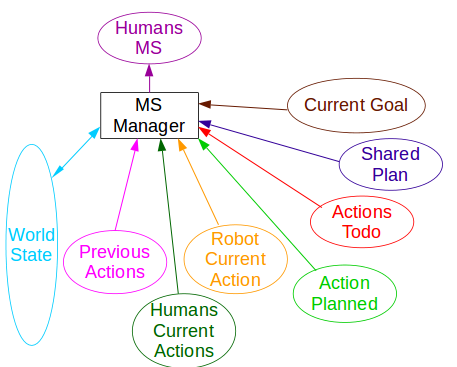
\includegraphics[width=0.5\textwidth]{figs/Chapter2/MSManager.png}
    \caption{Interaction of the Mental State Manager with the rest of the supervisor.}
    \label{fig:MSManager}
\end{figure}

\subsection{Robot Decision}

\begin{figure}[!h]
	\centering
    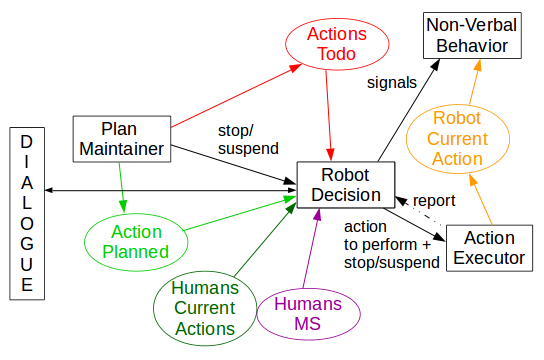
\includegraphics[width=0.7\textwidth]{figs/Chapter2/RobotDecision.png}
    \caption{Interaction of the Robot Decision module with the rest of the supervisor.}
    \label{fig:robotDecition}
\end{figure}

\subsection{Action Executor}

\begin{figure}[!h]
	\centering
    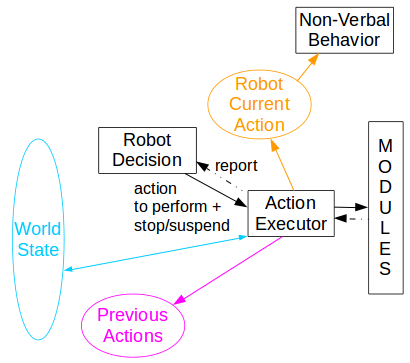
\includegraphics[width=0.5\textwidth]{figs/Chapter2/ActionExecutor.png}
    \caption{Interaction of the Action Executor with the rest of the supervisor.}
    \label{fig:actionExecutor}
\end{figure}

\subsection{Non-Verbal Behavior}

\begin{figure}[!h]
	\centering
    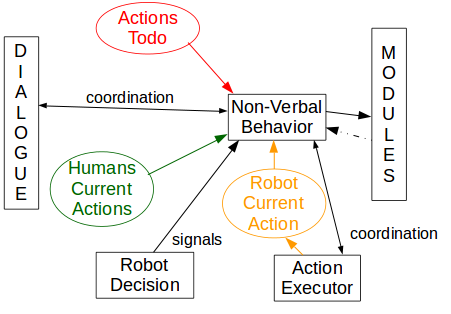
\includegraphics[width=0.5\textwidth]{figs/Chapter2/NVBehavior.png}
    \caption{Interaction of the Non-Verbal Behavior module with the rest of the supervisor.}
    \label{fig:NVBehavior}
\end{figure}

\section{Data representation}

\begin{itemize}
\item formalization data representation
\end{itemize}

\ifdefined\included
\else
\bibliographystyle{StyleThese}
\bibliography{These}
\end{document}
\fi
